\chapter{Réseaux de neurones récurrents}
\section{Motivation}
Nous avons pu voir que les réseaux feedforward peuvent être utilisés afin d'appendre à générer la sortie voulue en fonction de l'entrée du réseau. 
Néanmoins, ces réseaux sont limités à des entrées et des sorties de tailles fixes. De plus il ne peuvent gérer des réseaux présentant des cycles. On utilise alors des réseaux récurrents qui permettent un traitement plus efficace des séquences de données. On pourra ainsi faire de la prédiction et de la génération de séquence.

Dans un premier, nous verrons comment modéliser ces réseaux récurrents. Puis nous nous intéresserons à deux algorithmes d'optimisation permettant l'apprentissage des réseaux récurrents : Real Time Recurrent Learning (RTRL) et Back Propagation Through Time (BPTT).

\section{Dépliage}

Nous avons dit précédemment qu'un réseau de neurones récurrent est un réseau possédant des cycles. Néanmoins, il est difficile d'imaginer que la valeur de sortie d'un neurone au temps $t$ dépende de la sortie de ce même neurone au temps $t$. Pour résoudre ce problème, nous allons ajouter une dimension temporelle à nos réseaux et permettre aux neurones au temps $t$ de dépendre des valeurs d'autres neurones au temps $t-1$.

Afin de mettre en évidence cette dépendance temporelle sur nos graphes, les arêtes reliant la sortie d'un neurone au temps $t-1$ à un neurone au temps $t$ vont être annotées par un carré comme sur la figure \ref{arete_retard}. On les appelera arête "retard".

% Insérer figure avec une arête retard

On a alors de nouvelles équations pour la sortie du neurone $j$ :
\begin{equation}
\left\{
\begin{array}{ll}
t = 0, & y_j(t) = 0 \\
\forall t \geq 1, & y_{j}(t) = g_{j}(\sum_{i \in Pa_t(j)}{w_{ji}y_{i}(t)} + \sum_{i \in Pa_{t-1}(j)}{w'_{ji}y_{i}(t-1)})
\end{array}
\right.
\end{equation}
où $Pa_t(j)$ est l'ensemble des neurones ayant une arête allant vers $j$ au temps $t$ et $Pa_{t-1}(j)$ l'ensemble des neurones ayant une arête "retard" allant vers $j$.

Une manière commode de mettre en évidence cette dépendance temporelle est de déplier le graphe. 

% Insérer figure avec les instants t-1, t et t+1 d'un réseau

On peut même pour une séquence d'entrée donnée modéliser tous les calculs du réseau sans aucun cycle si on déplie le réseau un nombre suffisant de fois.

% Insérer figure avec le réseau déplier pour une séquence d'entrée

\section{BPTT}

Contrairement, à ce que nous avons fait lors du projet, nous allons d'abord présenter l'algorithme \textit{backpropagation through time} (BPTT) car il s'agit d'une simple généralisation de la rétropropagation déjà présentée pour les réseaux feedforward.

L'algorithme consiste en deux étapes :
\begin{enumerate}
\item Déplier le réseau récurrent pour avoir un réseau feedforward.
\item Appliquer l'algorithme de rétropropagation à ce réseau feedforward.
\end{enumerate}

La seule difficulté conceptuelle réside donc dans le dépliage.

\section{RTRL}

\section{Évaluation}

\subsection{Grammaire de Reber}

Dans un premier temps, nous comparerons ces algorithmes sur l'apprentissage de la grammaire de Reber, qui est régulière. Nous utiliserons la grammaire simple présentée sur la figure \ref{Grammaire de Reber simple}.

\begin{figure}[h!]
\begin{center}
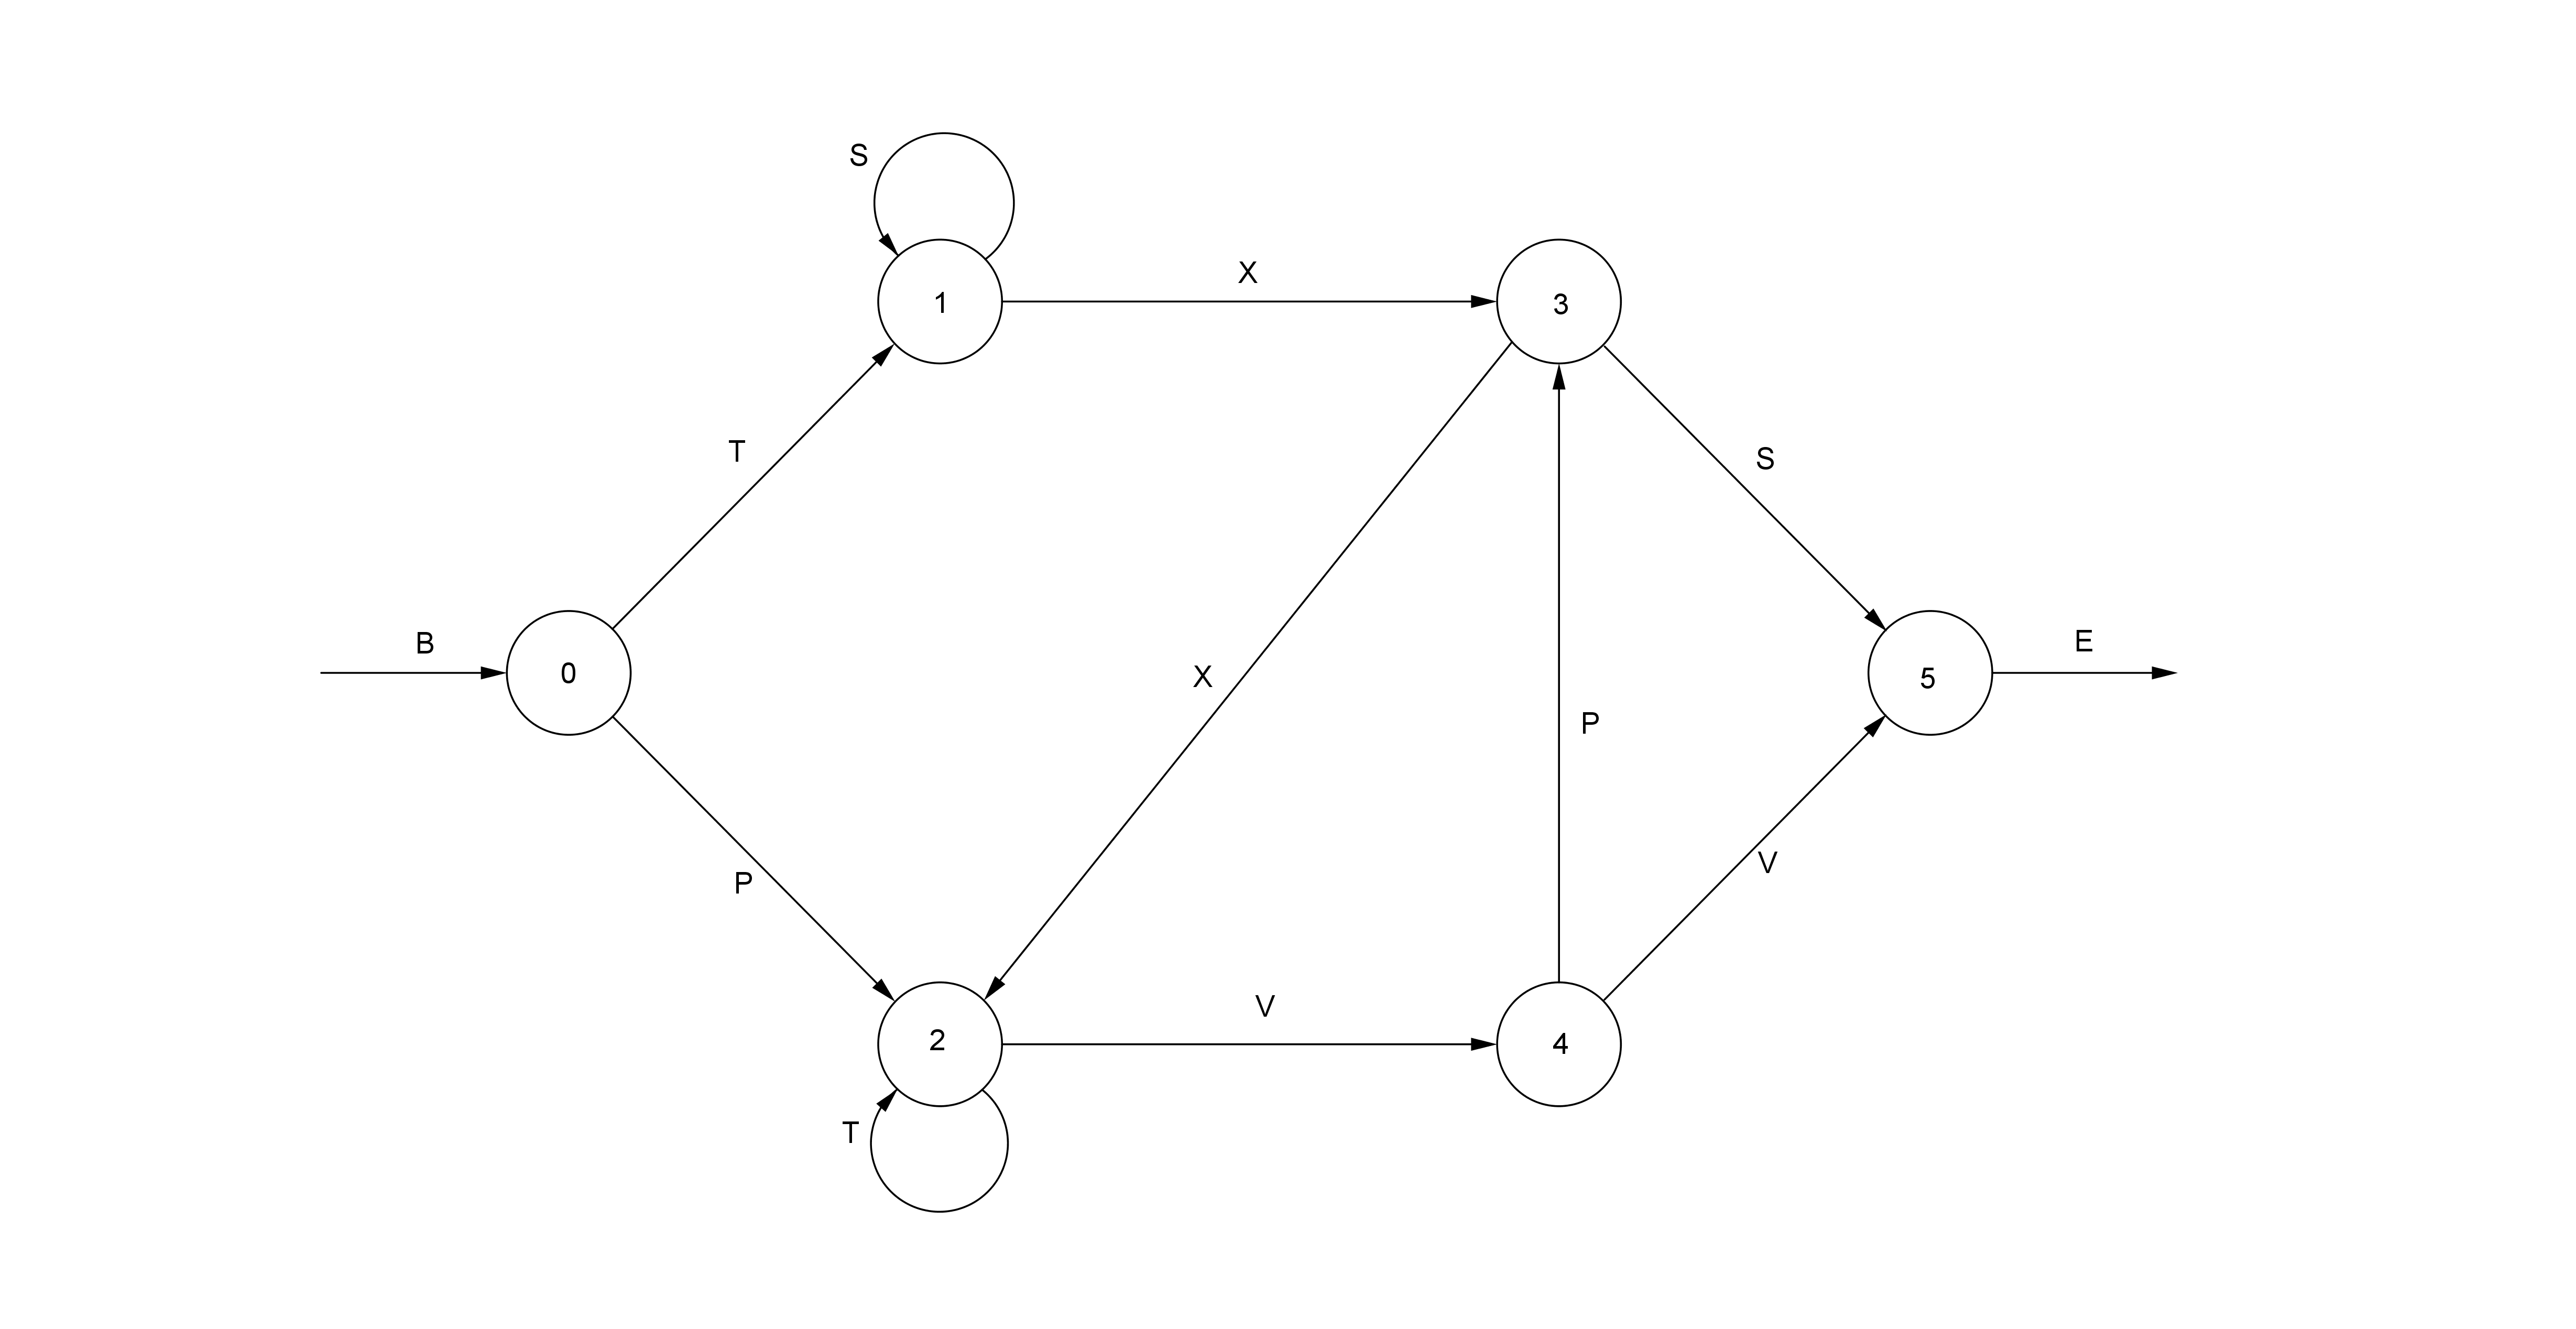
\includegraphics[scale=0.3]{images/reber_simple.png}
\caption{Automate reconnaissant la grammaire de Reber simple}
\label{Grammaire de Reber simple}
\end{center}
\end{figure}

A l'aide de cette automate, nous générerons deux ensembles de mots respectivement afin d'entraîner et de tester notre futur réseau. L'objectif du réseau sera alors d'apprendre cette grammaire afin de prédire les caractères possibles après un caractère donné.

L'étape suivante consistera à tester les algorithmes sur l'apprentissage de la grammaire de Reber symmétrique présentée sur la figure \ref{Grammaire de Reber symmétrique}.  
\begin{figure}[h!]
\begin{center}
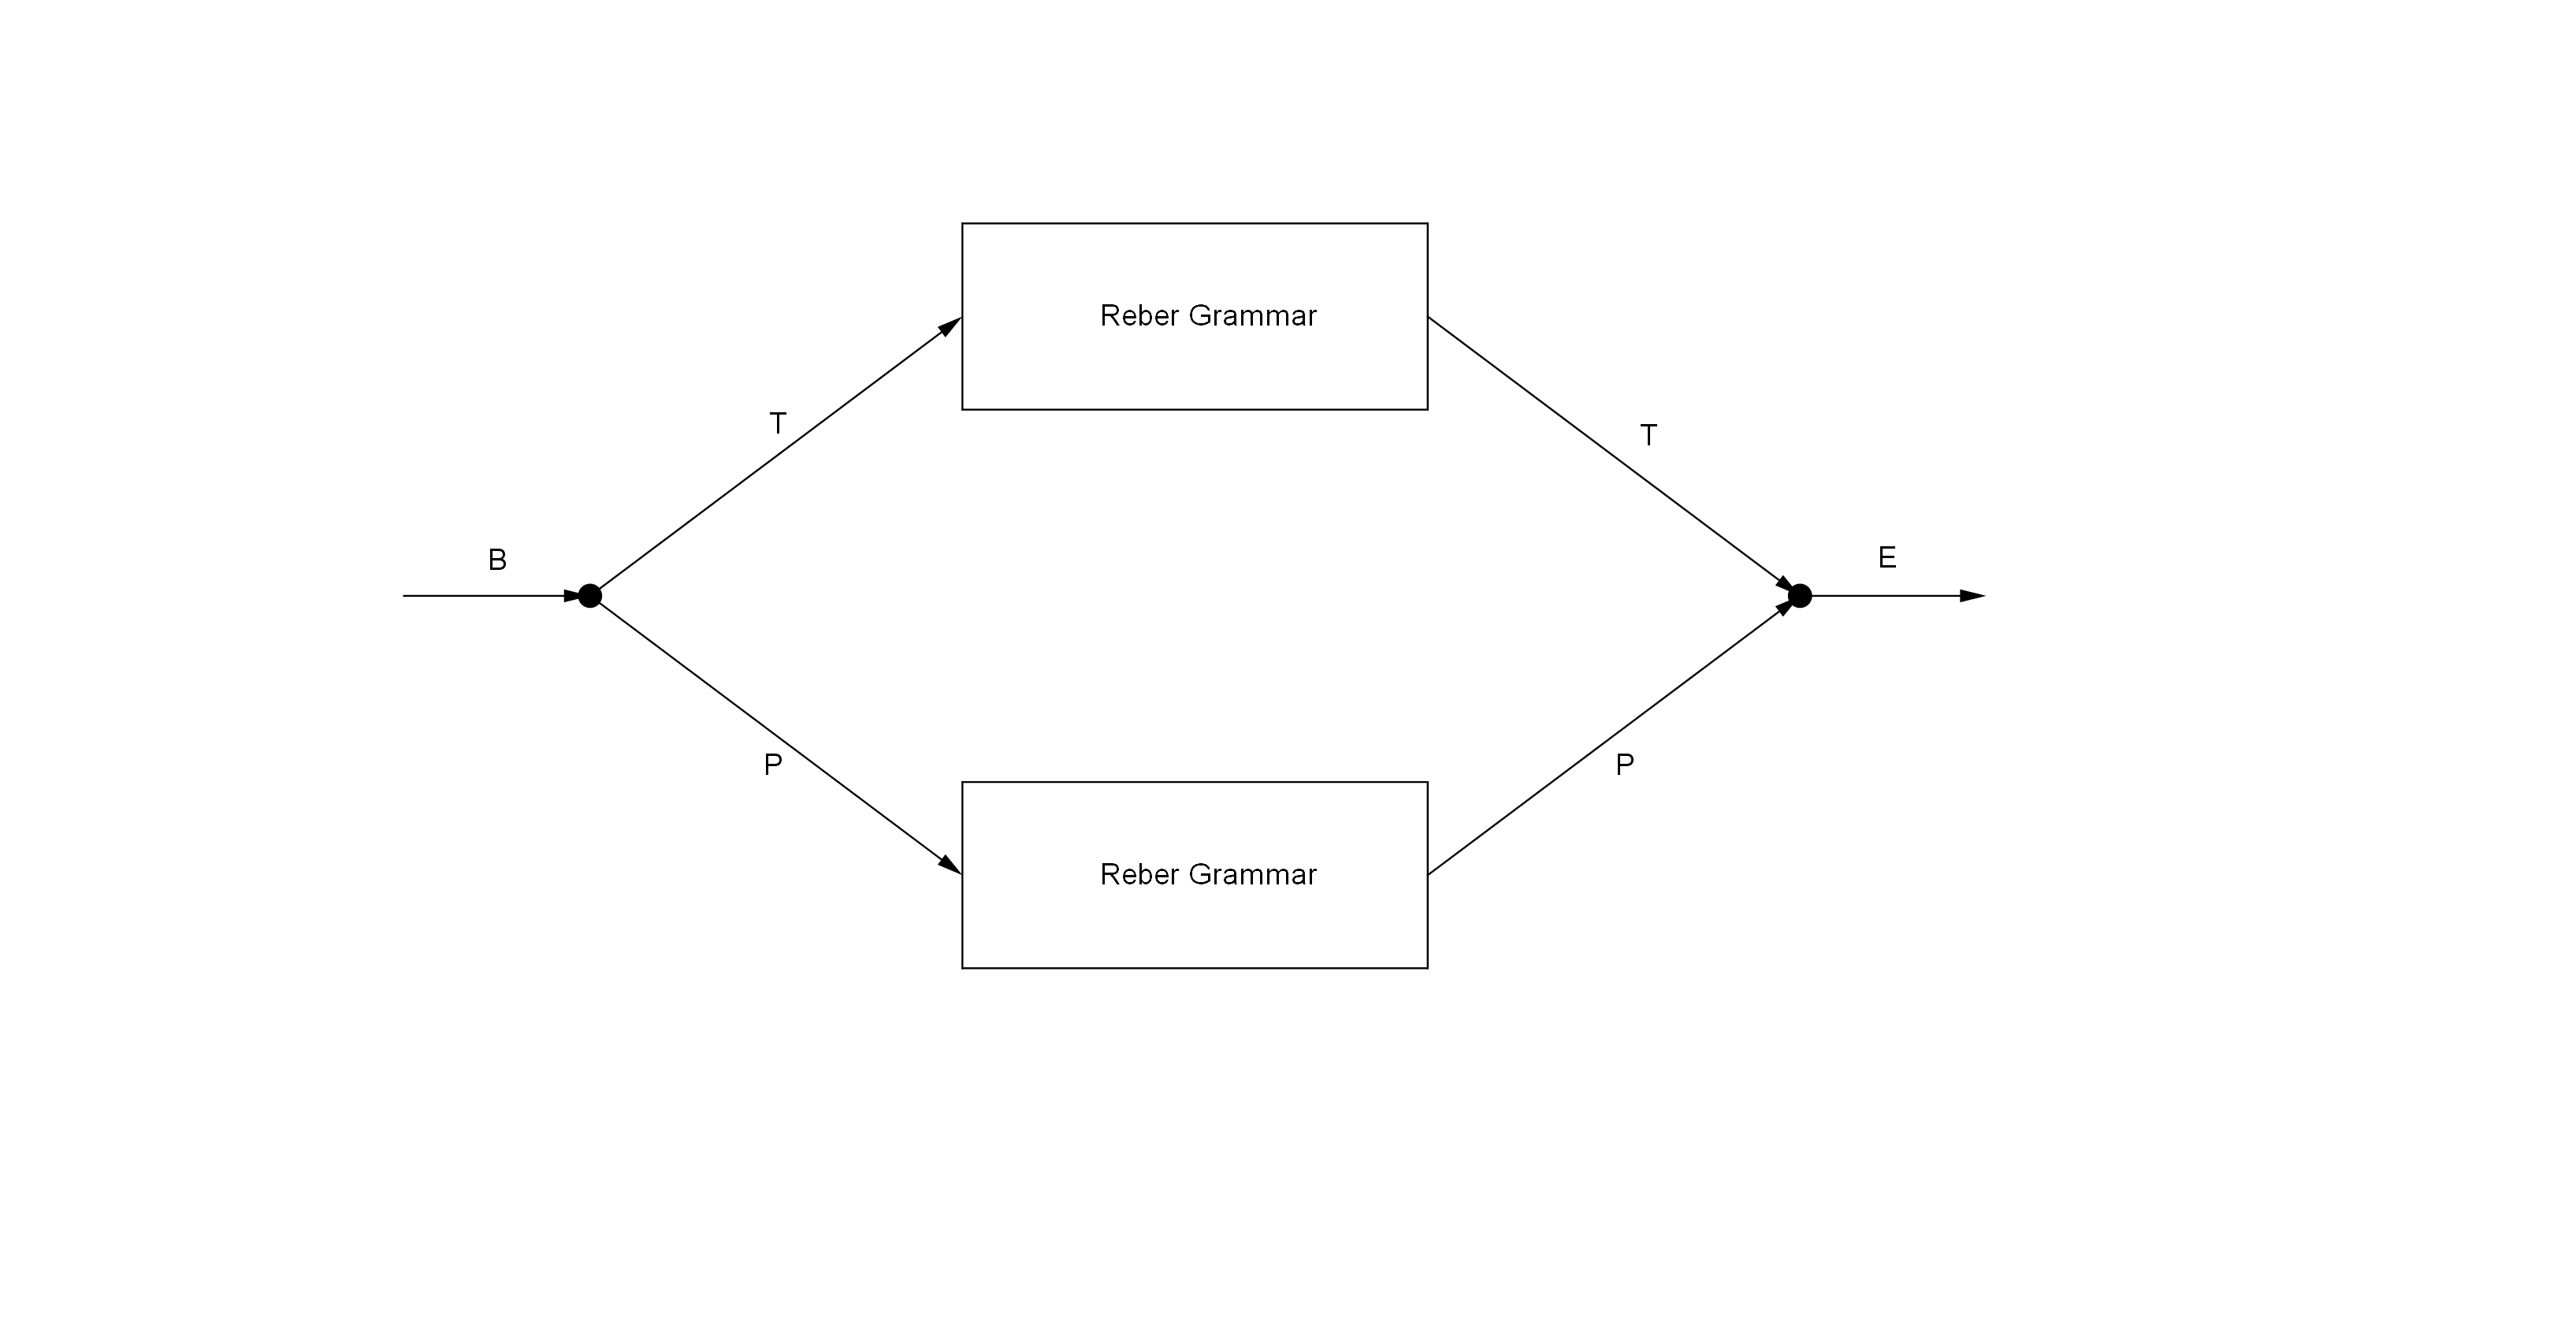
\includegraphics[scale=0.5]{images/reber_symmetrique.png}
\caption{Automate reconnaissant la grammaire de Reber symmétrique}
\label{Grammaire de Reber symmétrique}
\end{center}
\end{figure}

Dans cette situation, le réseau devra être capable de se souvenir d'un état passé (T ou P) afin de prédire le nouvel état (T ou P). Cet état passé pourra être plus ou moins lointain en fonction de la taille de la grammaire de Reber insérée au milieu. 

\section{Comparaison des deux algorithmes}

\section{Problème des dépendances temporelles}